%!TEX root = main.tex

\section{Use Case Study} 
\label{sec:usecase}

\begin{figure}[t] 
    \centering 
    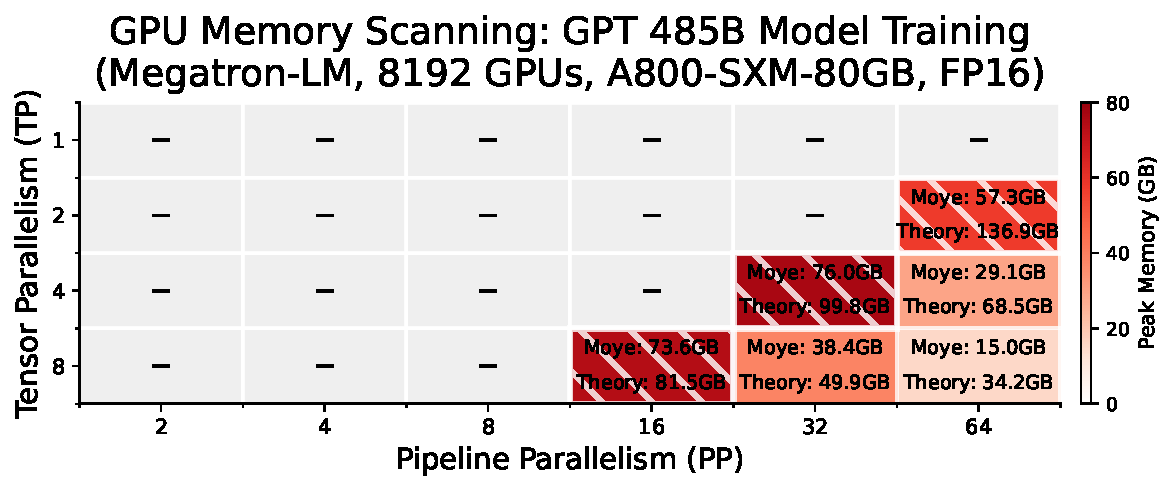
\includegraphics[width=1\linewidth]{figures/evaluation/memory_heatmap_485B_academic.pdf} 
    \vspace{-5mm}
    \caption{GPU memory constraint scanning for a 485B model on 8192 GPUs. Each cell represents a unique parallelism strategy defined by its PP and TP sizes, with DP implicitly set to satisfy PP * TP * DP = 8192. Gray cells indicate OOM conditions. The red, hatched cells highlight configurations that are empirically feasible yet are incorrectly identified as OOM by baseline analytical models.}
    \label{fig:memory_heatmap} 
    \vspace{-1em}
\end{figure}


\subsection{Use Case: Training Strategy Search} 
\label{sec:training-strategy-search}
\noindent A recurring practical question in large-scale training is: given a GPU cluster and the LLM, how should the training job and the parallelisms be configured to achieve the best efficiency? Answering this question by trial-and-error on the real cluster is prohibitively expensive, as each trial may waste thousands of GPU-hours. 
\sys provides a low-cost alternative by efficiently searching across a wide range of parallelism and system configurations. 

The workflow proceeds in two stages. 
First, \sys conducts a GPU memory feasibility scan via grid search over parallelism choices (see Figure~\ref{fig:memory_heatmap}). 
This step leverages its high-fidelity memory simulation to filter out infeasible configurations and avoid false OOM predictions that plague existing analytical models (e.g., Proteus, Calculon). 
Second, for all surviving candidates, \sys performs end-to-end simulation to estimate throughput and cost. 
By faithfully reconstructing the interaction between computation, communication, and memory behaviors, \sys enables accurate evaluation of training efficiency under each configuration. 
From these results, \sys recommends the configuration that minimizes time-to-train and monetary cost (see Table~\ref{tab:perf_time_cost_analysis}).




\begin{table}
    \centering
    \small
    \resizebox{0.48\textwidth}{!}{%
        \begin{tabular}{lcccc}
            \toprule
            \textbf{Setting} & \textbf{Peak memory} & \textbf{Throughput} & \textbf{Time (days)} & \textbf{Cost} \\
            \midrule
            \rowcolor{red!25}
            (PP16, TP8, DP64) & 73.6 GB & 455.8k tokens/s & 12.7 & \$2.45M \\
            \rowcolor{gray!25}
            (PP32, TP8, DP32) & 38.4 GB & 361.1k tokens/s & 16.0 & \$3.09M \\
            (PP64, TP8, DP16) & 15.0 GB & 331.9k tokens/s & 17.4 & \$3.36M \\
            (PP32, TP4, DP64) & 76.0 GB & 350.0k tokens/s & 16.5 & \$3.19M \\
            (PP64, TP4, DP32) & 29.1 GB & 222.1k tokens/s & 26.1 & \$5.02M \\
            (PP64, TP2, DP64) & 57.3 GB & 308.3k tokens/s & 18.8 & \$3.62M \\
            \bottomrule
        \end{tabular}
    } 
    \caption{Simulation results under different training configurations on 8,192 A800 GPUs for GPT 485B with a volume of 500B tokens. The training time is calculated using the total volume and predicted throughput, and the cost is derived accordingly using the market rent price of A800. The red row denotes \sys's choice, while the gray row is Calculon's choice which is suboptimal.}
    \label{tab:perf_time_cost_analysis}
    \vspace{-1.5em}
\end{table}


\yc{
\subsection{Use Case: Scaling-up Analysis} 
\label{sec:scale-up}
\begin{figure}[t]
    \centering
    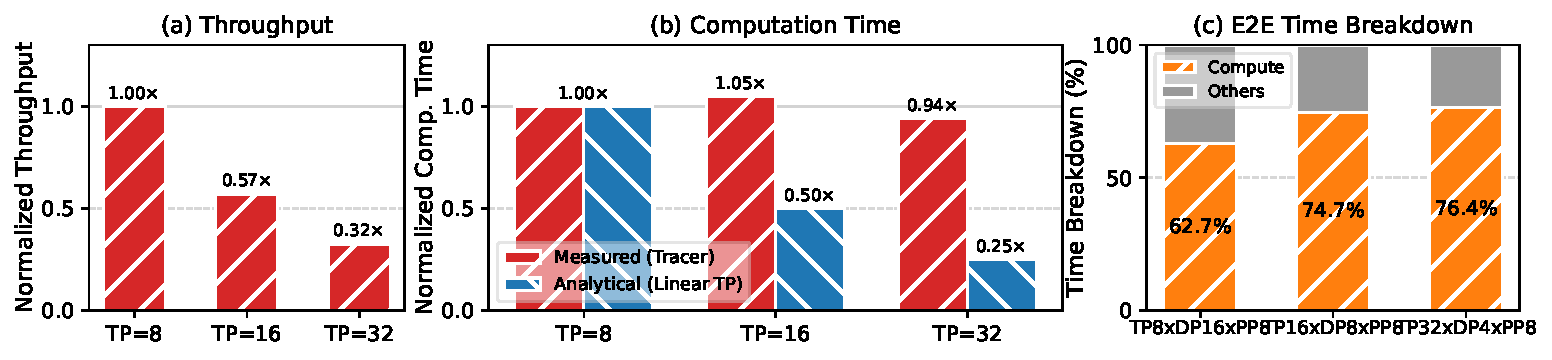
\includegraphics[width=1\linewidth]{figures/evaluation/tp_scaling_gpt175b_world1024.pdf}
    \vspace{-6mm}
    \caption{\yc{Scaling-up analysis for GPT-175B on 1,024 GPUs (fixed PP=8 and global batch size 256). \textbf{(a)} Normalized throughput under different TP degrees. \textbf{(b)} Normalized per-microbatch computation time from \sys's framework-specific ex-situ tracer versus an analytical model assuming ideal linear TP scaling. \textbf{(c)} Stage0 time breakdown into computation and \textit{others} across TP$\times$DP$\times$PP configurations.}}
    \label{fig:tp_scaling_gpt175b_world1024}
    \vspace{-1em}
\end{figure}

\noindent\textbf{Larger TP does not improve E2E throughput.}
A natural expectation is that scaling up TP to match more GPUs within a node can exploit fast NVLink/NVSwitch links and accelerate model-shard execution. We test this intuition on GPT-175B with 1,024 GPUs, fixed PP=8, and global batch size 256. Figure~\ref{fig:tp_scaling_gpt175b_world1024}(a) shows the opposite trend: normalized throughput drops from 1.0 at TP=8 to 0.57 and 0.32 at TP=16 and TP=32, corresponding to iteration time increasing from 34.4\,s to 60.5\,s and 106.2\,s. Thus, simply enlarging the TP domain can hurt rather than help end-to-end efficiency.

\noindent\textbf{Why it happens: TP increases, DP shrinks, but per-microbatch compute does not.}
Under fixed world size and PP, increasing TP compresses DP from 16 to 8 to 4, which increases the number of micro-batches per iteration from 16 to 32 to 64. This trade-off would be acceptable only if each micro-batch became proportionally cheaper. However, Figure~\ref{fig:tp_scaling_gpt175b_world1024}(b) shows that \sys's tracer measures nearly flat per-microbatch computation time: 1,349.7\,ms, 1,412.1\,ms, and 1,267.2\,ms for TP=8/16/32. In contrast, a naive analytical model assuming ideal linear TP scaling predicts 1,349.7\,ms, 674.8\,ms, and 337.4\,ms. Because the expected compute speedup never materializes, total stage0 computation rises sharply from 21.6\,s to 45.2\,s and 81.1\,s, which directly drives the throughput collapse.

\noindent\textbf{Takeaway for scaling-up decisions.}
Figure~\ref{fig:tp_scaling_gpt175b_world1024}(c) confirms that computation dominates the bottleneck stage across TP8$\times$DP16$\times$PP8, TP16$\times$DP8$\times$PP8, and TP32$\times$DP4$\times$PP8: its share grows from 62.7\% to 74.7\% and 76.4\%, while \textit{others} remain non-trivial. Therefore, once memory feasibility is satisfied, TP should be treated as a tunable parameter rather than maximized by default; when larger TP only reduces DP and increases micro-batching, additional scale-up can reduce throughput. This use case highlights the value of \sys's high-fidelity tracing inputs for exposing non-ideal scaling and guiding reliable LLM training configuration decisions.
}